% !TeX spellcheck = cs_CZ
% RA_exam01.tex
\begin{example}
  Navrhněte graficko-početní metodou ve Smithově diagramu přizpůsobovací obvod pro 
  \(Z_L = \SI{30 - 65j}{\ohm}\) , \(Z_S = 50\)  a \(f = \SI{100}{\MHz}\).
  
  \textbf{Řešení:}
  Platí \(z_L = \dfrac{Z_L}{Z_S} = \num{0.6000 - 1.3000j}\), daný bod se tedy nachází ve 
  \textbf{4. kvadrantu}, \textbf{vně} kružnice konstantní reálné části impedance \(r = 
  1\). Proto volíme strukturu typu \(H\) viz. obr. \ref{RA:fig_smith02}. 
  \newline
  \begin{itemize}
    \item 1. krok: Začínáme v admitančních souřadnicích. Pro posun z bodu \(y_L = 
          \dfrac{1}{z_L} = \num{0.2927 + 0.6341j}\) nejkratší cestou na kružnici \(r = 1\), 
          tj. do bodu \(y_1 = \num{0.2927 + 0.4500j}\), musíme z admitance \(y_L\) ubrat 
          normovanou susceptanci \(\num{0.6341} - \num{0.4500} = \num{0.1841} = \Delta b = 
          \dfrac{\omega L_2}{Z_0}\). Paralelní indukčnost \(L_2\) tedy bude
          \MULTIPLY{2}{\numberPI}{\nmbrA}
          \MULTIPLY{\nmbrA}{100}{\nmbrB}
          \MULTIPLY{\nmbrB}{0.1841}{\nmbrC}
          \DIVIDE{50}{\nmbrC}{\nmbrD}
          \MULTIPLY{1000}{\nmbrD}{\nmbrE}
          \ROUND[2]{\nmbrE}{\sol}
          \begin{equation*}
            L_2 = \frac{Z_0}{\omega\abs{\Delta b}} = 
                  \frac{50}{2\cdot\pi\cdot\num{100e6}\cdot\num{0.1841}} = \SI{\sol}{\nano\henry}
          \end{equation*}
    
           {\centering   %\ref{RA:fig_RA_ADS_smith01} 
            \captionsetup{type=figure}
            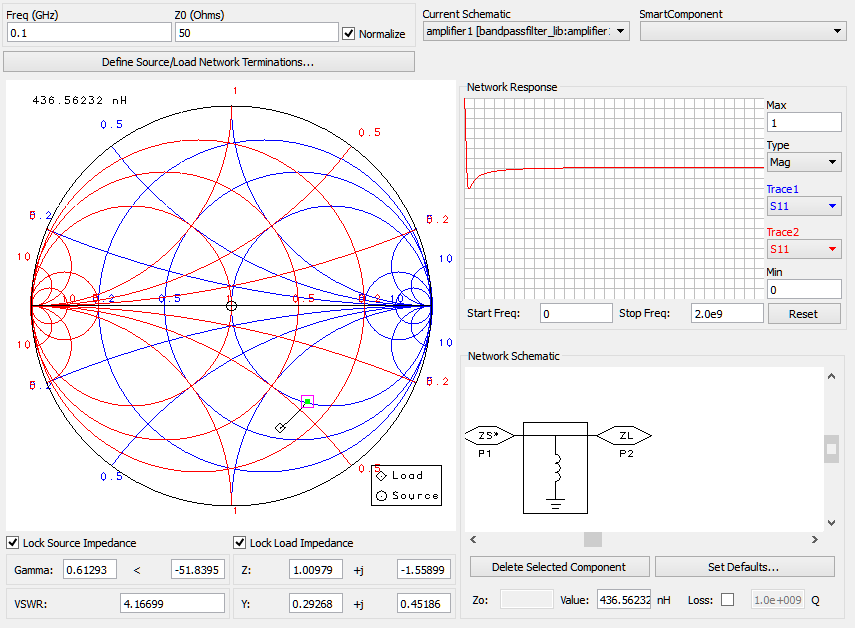
\includegraphics[width=0.8\linewidth]{ADS_smith01.png}
            \captionof{figure}{ADS Smith Chart tool: Přechod z bodu \(y_L \rightarrow y_1\)}
            \label{RA:fig_ADS_smith01} 
            \par}
          
    \item 2.krok: Pro posun z bodu \(z_1 = \dfrac{1}{y_1} = \num{1 - 1.5479j}\) do bodu 
          \(z_S = \num{1 + 0j}\) musíme k \(z_1\) přidat normovanou reaktanci \(1.5479 = \Delta 
          x = \frac{\omega L_2}{Z_0}\). Sériová indukčnost \(L_1\) tedy bude
          \MULTIPLY{2}{\numberPI}{\nmbrA}
          \MULTIPLY{\nmbrA}{100}{\nmbrB}
          \MULTIPLY{50}{1.5479}{\nmbrC}
          \DIVIDE{\nmbrC}{\nmbrB}{\nmbrD}
          \MULTIPLY{1000}{\nmbrD}{\nmbrE}
          \ROUND[2]{\nmbrE}{\sol}
          \begin{equation*}
            L_1 = \frac{\Delta x Z_0}{\omega} = 
                  \frac{\num{1.5479}\cdot\num{50}}{2\cdot\pi\cdot\num{100e6}} = 
                  \SI{\sol}{\nano\henry}
          \end{equation*}
           
           {\centering   %\ref{RA:fig_RA_ADS_smith02}
            \captionsetup{type=figure} 
            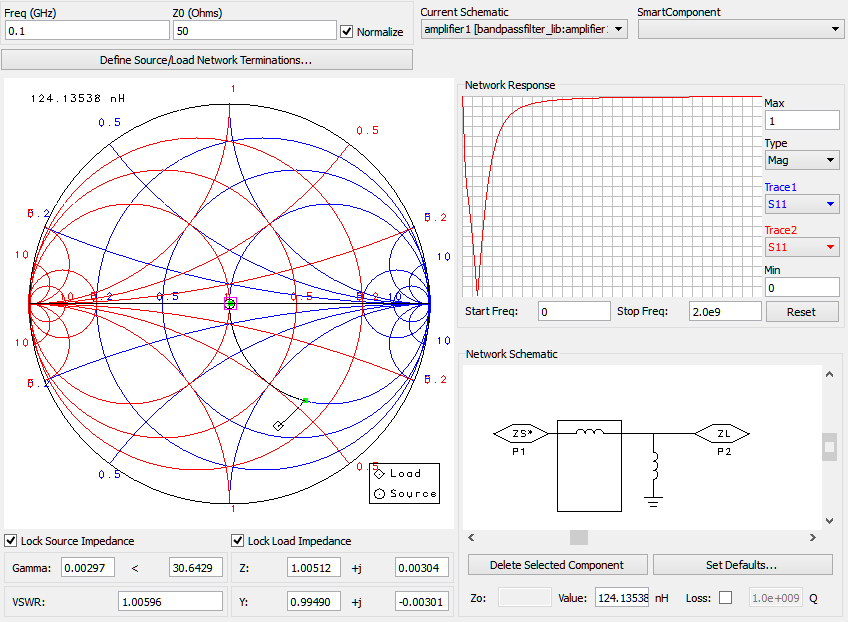
\includegraphics[width=0.8\linewidth]{ADS_smith02.png}
            \captionof{figure}{ADS Smith Chart tool: Přechod z bodu \(z_1 \rightarrow z_S\)}
            \label{RA:fig_ADS_smith02} 
            \par} 
  \end{itemize}
\end{example}